\section{Mission}
Le sujet de l'alternance était d'approfondir la culture \emph{DevOps} en mettant en relation avec Ansible, Docker, Jenkins et le cloud avec Amazon AWS sur un rythme Agile \textit{Scrumban} en ayant Python comme langage de base.

Comme nous avons déjà vu dans la Section \ref{bcd}, le complément BCD est celui qui aide à implémenter les bonnes pratiques DevOps au client grâce à l'automatisation de la création d'environnements et l'approvisionnement de stack Bonita, et aussi la compilation et déploiement d'un application Bonita.

À continuation, nous allons voir les concepts \emph{DevOps} ciblés par l'applicatif pour donner un cadre théorique, puis on verra plus en détail la travail fait cette année d'alternance.

\subsection{Devops}\label{sec:devops}
De nos jours, dans le domaine du numérique, nous livrons une large gamme de services grâce à des expériences numériques, et pour les améliorer, nous devons avoir le retour du client pour pouvoir proposer de nouveaux types d’expériences et de valeurs. Ce faisant, nous allons être plus compétitifs et nous aurons des nouveaux moyen d'interagir avec les clients.

Tout cela, nous pouvons le faire grâce à des bonnes pratiques pour rendre le travail beaucoup plus efficace, pour cela nous allons entrer dans le monde DevOps.

DevOps est avant tout une culture, des pratiques collaboratives et de l'automatisation qui alignent les équipes de développement et d'opération afin qu'elles puissent améliorer leur expérience client, répondre plus rapidement aux besoins et assurer l'innovation \cite{IsaacSacolick2016DrivingCulture}.

Cependant, cela n'est pas seulement une culture, DevOps involucre principalement un changement de base de comment nous gérons nos applications et comment nous les déployions, en investissant dans l'automation et en changeant les application héritées \cite{benjamin_wootton}.

Pour cette raison, quand nous parlons de DevOps, nous avons:

\begin{itemize}
\item L'automatisation de test.
\item Assurer des déploiements plus fréquents et plus fiables.
\item Avoir la clarté de rôles et des responsabilités.
\item Définir l'indicateur de performance \(KPI\) et sa portée.
\item Automatisation et surveillance.
\end{itemize}

Pour commencer, nous devons nous assurer que tous sont alignés sur ce que DevOps signifie et avec un défi et non à l’ensemble des pratiques DevOps.

Nous devons également rester concentrés sur l’assurance qualité (QA) en sachant qu’il s’agit d’une discipline et d’un ensemble de compétences distincts.

Par exemple, dans la Figure \ref{devops_operational_model} nous voyons une modèle opérationnel proposé ou dans la partie supérieur, l'équipe de \textbf{Dev} qui travaille en \textit{Sprint} en développant les \textit{Epics} avec l'objectif de livrer (Release) les nouvelles fonctionnalités. Dans l'autre côté, l'équipe de \textit{Ops} centré en les issues, l'architecture, la sécurité et les transmettre comme défauts (Defects).


\begin{figure}[!ht]
\centering
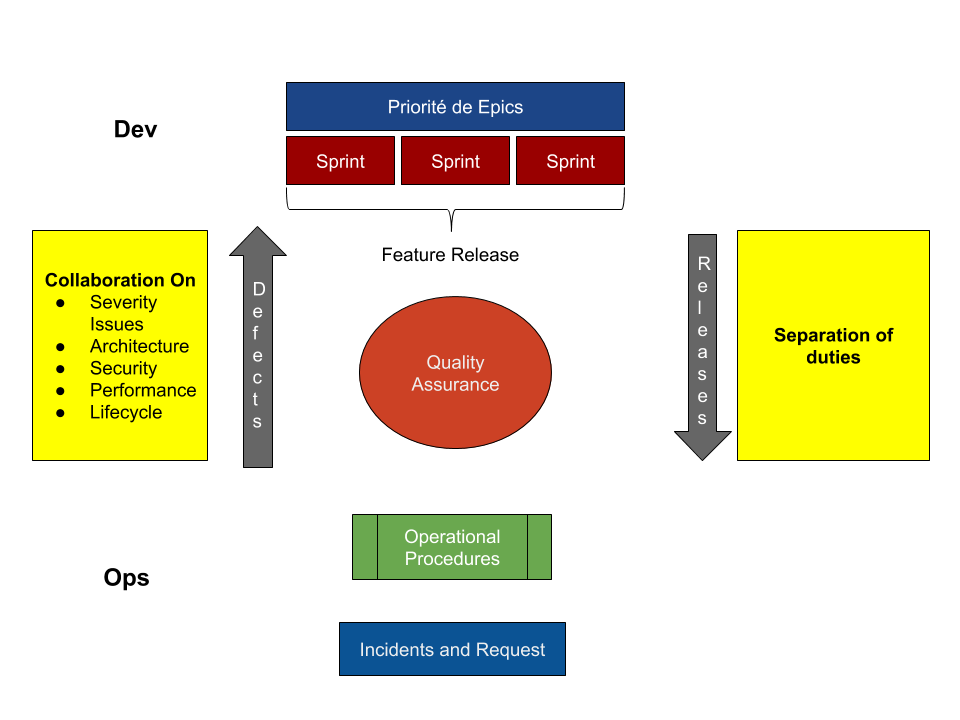
\includegraphics[scale=0.45]{devops_operational_model.png}
\caption{Modèle Opérationnel \cite{IsaacSacolick2016DrivingCulture}}
\label{devops_operational_model}
\end{figure}


\subsubsection{Acteurs}
Dans la Figure \ref{devops_operational_model} nous voyons trois acteurs principaux dans cette conversation:

\subparagraph{QA}
C'est une équipe composée par des personnes avec distinctes disciplines qui doivent travailler avec \textit{Dev} pour développer et automatiser les test.
\subparagraph{Dev} L'équipe doit livrer les livrables avec des \emph{runbooks} et d'assurer que les amélioration opérationnelles sont priorité.
\begin{itemize}
  \item Le 30\% d'un sprint doit cibler des défets téchniques.
  \item Cibler le \emph{développement complet}, c'est-à-dire, le développement prêt pour les tests de \textit{QA}.
  \item Collabore activement avec \textit{Ops}.
  \item Assurer que l'application récolte des données qui aident à l'amélioration.
\end{itemize}
\subparagraph{Ops}
L'équipe doit fournir des services dans le cloud pour permettre \textit{Dev} être plus agile et lui permettre d'apprendre à résoudre la plupart des problèmes de production.


\subsection{Le Défi}
Dans la Section \ref{sec:devops}, nous avons listé les activités de transition DevOps qui sont aussi des pratiques que \emph{BCD} vise à donner aux clients de Bonita. Figure \ref{fig:dev-to-prod}

\begin{figure}[!ht]
\centering
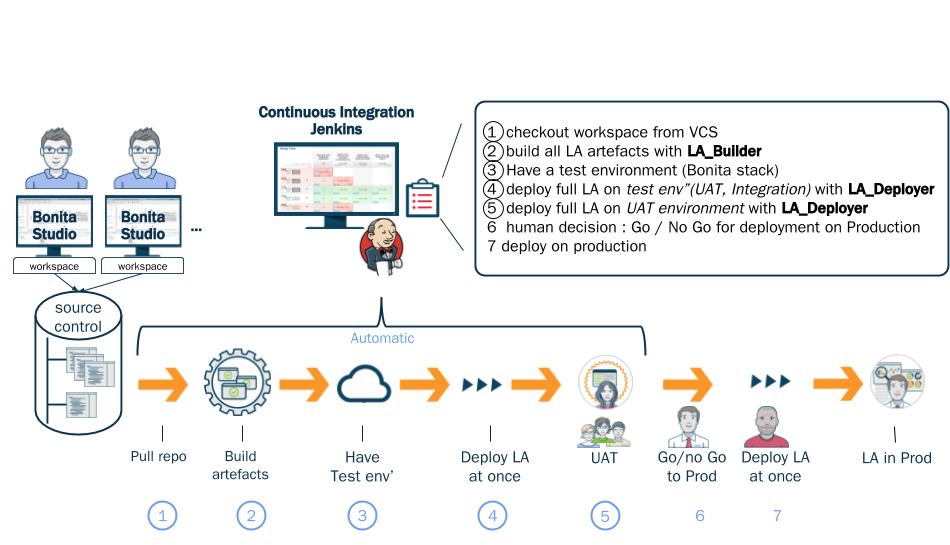
\includegraphics[width=\textwidth,keepaspectratio]{dev-to-prod.png}
\caption{Dev à Prod}
\label{fig:dev-to-prod}
\end{figure}

Les technologies utilisées actuellement sont:
\begin{itemize}
  \item Ansible
  \item Python
  \item Docker
  \item Jenkins
  \item Cloud (AWS)
\end{itemize}

Pour cette mission, j'ai dû approfondir mes connaissances sur:
\subparagraph{DevOps} De nouvelles approches qui incluent l'Intégration Continue (CI), le Déploiement Continu (CD).
\subparagraph{Agile} La communication dans un environnement agile avec les rituels.
\subparagraph{Python} Comme un langage complet avec le paradigme OO avec TDD comme méthodologie.
\subparagraph{Docker} Les bonnes pratiques pour créer une image, et comment nous pouvons les utiliser pour déployer plus rapidement des applications.
\subparagraph{Jenkins} L’architecture et le langage DSL pour  créer des "jobs" et "pipelines" pour automatiser les tests, la compilation, l’empaquetage d'un produit final.
\subparagraph{AWS} Tous les nombreux services et la façon de nous en servir.


\subsection{Travail réalisé}\label{sec:work_done}
Nous avons vu dans dans la Figure \ref{frame_safe} le chemin suivi pour la création et la définition des \textit{Epics}, \textit{Millestones} et le \textit{Backlog}. Dans la Figure \ref{fig:backlog} nous pouvons regarder un exemple du contenu Backlog.

Pendant le déroulement de mon alternance, j'ai travaillé sur plusieurs items du \textit{Backlog}. Appendice  \ref{appen:my_backlog}. Chaque item était bien découpé de sorte que la tâche puisse se terminer dans le délai d'un \textit{Sprint}.

\begin{figure}[!ht]
\centering
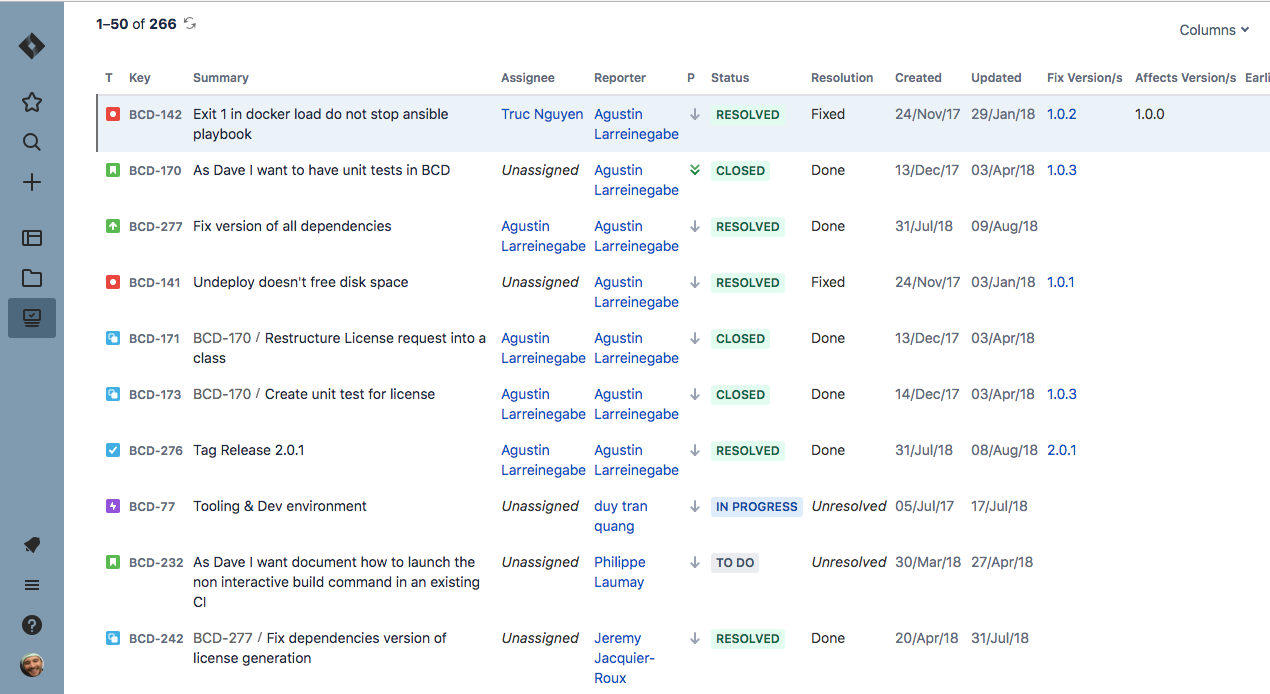
\includegraphics[width=\textwidth,keepaspectratio]{backlog.png}
\caption{Exemple Backlog}
\label{fig:backlog}
\end{figure}

Pour cela, je devais effectuer des actions différentes comme:

\subparagraph{Python} Développer et maintenir les scripts du Command Line Interface (CLI) de BCD.
\begin{itemize}
  \item J'ai participé à la réorganisation du code pour le rendre plus modulaire.
  \item J'ai participé à l'élaboration des tests unitaires pour le module BCD.
  \item J'ai participé au développement du module de \enquote{Licensing}.
\end{itemize}

\subparagraph{AWS} Une partie de BCD gère des instances dans le cloud, aussi l'entreprise a passé d'autres services sur le cloud.
\begin{itemize}
  \item J'ai aidé à implémenter le service \enquote{Organization} de AWS.
  \item J'ai dû m'impliquer plus dans les services EC2, Lambda, S3, RDS.
\end{itemize}

\subparagraph{Ansible} Développer et maintenir des \enquote{Playbook} Ansible.
\begin{itemize}
  \item J'ai participé à l'adaptation des scripts pour supporter le nouveau dépôt privé d'images docker.
\end{itemize}

\subparagraph{Jenkins} Exécution de jobs pour l'empaquetage de livrables.

\subparagraph{Git} Gestion du dépôt privé.
\begin{itemize}
  \item Revue de \enquote{Pull Request}
  \item \enquote{Merge} dans la branche correspondante.
  \item \enquote{Tag} et livre des nouvelles versions.
\end{itemize}

\subparagraph{Docker} Maintenir des images et l'investigation des nouvelles caractéristiques.

\subparagraph{Activités collatérales} Pour mieux organiser le travail en équipe, nous suivons des rituels Agile
\begin{itemize}
  \item Le \enquote{Daily Meeting} pour faire le point sur les tâches effectuées et communiquer sur les difficultés rencontrées.
  \item La \enquote{Rétrospective}, pour s’améliore.
  \item La \enquote{Réunion hebdomadaire},  elle réunit toutes les parties prenantes du projet pour faire le point sur son avancement. Ainsi, tous les participants peuvent se rendre compte si l’état du projet correspond à leurs besoins, attentes ou objectifs.
  \item \enquote{Les estimations}, où nous faisons des hypothèses à échelle relative, pour estimer une charge de travail par exemple. Cette réunion est importante pour déterminer correctement la complexité et la valeur apportée de la tâche à réaliser pour effectuer une estimation de bonne qualité.
  \item \enquote{La sélection}, où nous déterminons efficacement la charge de travail à accomplir définie dans le backlog lors de l'itération.
\end{itemize}

\subsubsection{Gestion de risques}
Il y a toujours plusieurs risques associés au développement du logiciel. Dans cette sous-partie, nous allons voir quelques risques que j'ai vu s'atténuer en comparaison à d'autres expériences de travail (pas Agile). \cite{basile_plessis_2014}
\begin{center}
\begin{tabular}{p{3cm}|p{3cm}|l|l|p{5cm}}
Description & Conséquence & Probabilité & Impact & Action \\ \hline
Prévision de travail pas juste & Rien livrer du tout & Faible & Fort & Le \enquote{Daily Metting} permet de s'assurer que sa prévision de \enquote{Sprint} est toujours d'actualité \\
Baisse de qualité du code & Bogue introduit & Modéré & Fort & Mise en place de CI, revues de code avant de l'ajouter dans la branche principale, test unitaire \\
Perte d'engagement de l'équipe & Équipe démotivée, et baisse de performance & Faible & Fort & La \enquote{Retrospective} suite de chaque \enquote{Sprint} aide l'équipe à s'améliorer. \\
Incompréhension des fonctionnalités & Ne pas livrer les bonnes fonctionnalités ou celles qui n'apportent pas de valeur & Faible & Modéré & Le \enquote{Spring Planning} permet à l'équipe de choisir les \enquote{stories} et s'engager. \\


\end{tabular}
\end{center}


\subsection{Travail qui reste}
Nous avons dit que BCD est né d'un besoin interne et des retours de clients, c'est ainsi que les fonctionnalités demandées augmentent et que le produit est toujours en évolution pour fournir au client une meilleure expérience quand il développe avec Bonita. Appendice \ref{appen:backlog}


\subsection{Les Compétences acquises}
Nous avons dans la Section \ref{sec:work_done} les outils et technologies que j'ai eu l'opportunité de toucher du doigt.
Pourtant, je ne peux pas dire que j'aie approfondi seulement le côté technologique et technique, parallèlement, j'ai amélioré mes aptitudes communicatives.


\subsection{Bilan}
Cette période d'alternance chez Bonitasoft m'a apporté une nouvelle expérience professionnelle. Grâce à cette année, j'ai acquis de nouvelles connaissances autant dans le domaine fonctionnel que dans les techniques.

Parmi les difficultés rencontrées, le travail sur un code qui existait déjà avec un langage que je ne connaissais pas en profondeur. L'acquisition des connaissances sur les nouvelles techniques et  technologies ont été aussi une entrave mais à la fois, un défi intéressant et enrichissant qui m'a beaucoup plu.

Cette expérience m'a permis d'affuter mes compétences grâce à l'intégration dans une équipe humaine et dynamique qui a été un véritable catalyseur et une source inépuisable de connaissances et d'expériences.


\subsection{Réflexion finale}
Cette formation en alternance m'a permis d'obtenir beaucoup de compétences et de savoir-faire, que ce soit sur le plan informatique avec la multitude de nouvelles technologies abordées, ceci s'ajoutant aux connaissances déjà acquises que j'ai pu approfondir. Mais également sur le plan personnel, toute la confiance qui, dès mon arrivée, m'a été donnée par l'équipe ; ma liberté d'expression et de prise de décisions ainsi que le partage d'expériences avec les collègues ont été très enrichissants et formateurs.

